\documentclass[12pt]{beamer}
\usepackage[utf8]{inputenc}
%\usepackage[francais]{babel}
\usepackage[T1]{fontenc}
\usepackage{lmodern, marvosym, graphicx, multicol, lastpage}
\usepackage{geometry}
%\usepackage[hyperindex=true, colorlinks=true, breaklinks=true, linkcolor=blue]{hyperref}
\usepackage{fancyhdr, verbatim}
%\usepackage{pgf/pgf}
%\usepackage{pgf-pie-0.2.1/pgf-pie}

%\geometry{hmargin=1.5cm, vmargin=2cm}
%\addtolength{\parskip}{8pt}



\defbeamertemplate*{footline}{infolines theme}{
	\leavevmode%
		\hbox{%
				\begin{beamercolorbox}[wd=.43\paperwidth,ht=2.25ex,dp=1ex,center]{title in head/foot}%
				\usebeamerfont{title in head/foot}\insertshorttitle
				\end{beamercolorbox}%
				\begin{beamercolorbox}[wd=.50\paperwidth,ht=2.25ex,dp=1ex,center]{date in head/foot}%
				\usebeamerfont{date in head/foot}\insertshortdate{}%
				\end{beamercolorbox}%
				\begin{beamercolorbox}[wd=.07\paperwidth,ht=2.25ex,dp=1ex,left]{page in head/foot}%
				\insertframenumber{} / \inserttotalframenumber
				\end{beamercolorbox}
		}
}
\setbeamerfont{title}{series=\bfseries,size=\huge}
\setbeamerfont{subtitle}{series=\it,size=\huge}

%\usebackgroundtemplate{\includegraphics[width=\paperwidth]{img/background.jpg}}

\newcommand{\titreA}{B.H. Consulting\\Authentication}
\newcommand{\titreB}{Industrial project}
%

\renewcommand{\headrulewidth}{1pt} %thikness of the line under our names
\lhead{\textbf{\titreA{} (\titreB)}}
\rhead{\emph{BOUGET / GUÉPIN / PINHÈDE / VAUBOURG}}
\lfoot{TELECOM Nancy - PI}
\cfoot{\thepage{} / \pageref{LastPage}}
\rfoot{2012-2013}

\title{\titreA}
\subtitle{\titreB}
\author{Nicolas BOUGET, Julien GUÉPIN, Marc~PINHÈDE,~Julien~VAUBOURG}
\institute{TELECOM Nancy}
\date{December 20, 2012}
\titlegraphic{\includegraphics[width=60pt]{img/BHConsulting.jpg}\hfill\includegraphics[width=80pt]{img/ul.png}\hfill\includegraphics[width=70pt]{img/telecom-nancy.jpg}}

\begin{document}
\begin{frame}
\titlepage
\end{frame}

\begin{frame}{Introduction}
    \begin{itemize}[<+->]
	\item \emph{TELECOM Nancy} \textbf{third year} biggest project
	\vfill
	\item \textbf{Multiple supervisors}
	\vfill
	\item \textbf{Intermediate} presentation
	\vfill
	\item Overview of the \textbf{situation and progression}
    \end{itemize}
\end{frame}

\begin{frame}
    \frametitle{Outline}
    \begin{enumerate}
	\item \large{Context}
	\vfill
	\item \large{Work organization}
	\vfill
	\item \large{Technical situation}
    \end{enumerate}
\end{frame}

\part{Context}
\frame{\partpage}
\section{Context}

\begin{frame}{TELECOM Nancy}
    \begin{center}
    \includegraphics[width=100pt]{img/telecom-nancy.jpg}
    \end{center}
    \begin{itemize}[<+->]
	\item MSC in Computer Science, like a french "Grande école"
	\vfill
	\item Accredited bt the Engineer Qualification Commitee (CTI)
	\vfill
	\item Formerly named \textbf{ESIAL}, changed its name in 2012\\
    \end{itemize}
\pause
\vfill
\begin{center}
\textbf{IL \hfill\pause LE \hfill\pause SIE \hfill\pause TRS}
\end{center}
\end{frame}

\begin{frame}{Industrial project}
    \begin{itemize}[<+->]
    \item \textbf{4 students} working for a company\vfill
    \item \textbf{12 hours a week} (about 250 hours per student)\vfill
    \item Use of a \textbf{real project} procedure\vfill
    \item Tackles every aspect of a project\vfill
    \item A good opportunity to discover how to manage a project\vfill
    \end{itemize}
\end{frame}

\begin{frame}{B.H. Consulting}
    \begin{center}
	\includegraphics[width=100pt]{img/BHConsulting.jpg}
    \end{center}

    \begin{itemize}[<+->]
    \item Created by \textbf{Bertrand PÉTAT} in 2000\vfill
    \item \textbf{Human-scaled} firm working in network implementation\vfill
    \item Five employees\vfill
    \end{itemize}
\end{frame}

\begin{frame}{B.H. Consulting}
\vfill
    \begin{figure}
	\includegraphics[width=300pt]{img/organigramme_en.pdf}
    \end{figure}
\vfill
\end{frame}

\begin{frame}{Project motivations}
    \begin{itemize}[<+->]
	\item Set up a \textbf{network access control}
	\vfill
	\item Simplify \textbf{access right} management
	\vfill
	\item \textbf{Avoid repetitive tasks}
    \end{itemize}

\end{frame}
    
\part{Work organization}
\frame{\partpage}
\section{Work organization}

\begin{frame}{Team presentation}
    \begin{itemize}[<+->]
	\item {\bf Julien GUÉPIN} - \emph{Software Engineering}
	\vfill
	\item {\bf Marc PINHÈDE} - \emph{Embedded Software}
	\vfill
	\item {\bf Julien VAUBOURG} - \emph{Telecoms, Networks and Services}
	\vfill
	\item {\bf Nicolas BOUGET} - \emph{Telecoms, Networks and Services}
    \end{itemize}
\end{frame}

\begin{frame}{VM Project}
    \begin{center}
    \includegraphics[width=160pt]{img/vmproject_logo.png}
    \end{center}
    \begin{itemize}[<+->]
	\item Software used to \textbf{assist the team}
    	\vfill
    	\item Assist the project leader to \textbf{follow task progress}
    	\vfill
    	\item \textbf{Gantt diagram} auto-generation
    	\vfill
    	\item \textbf{Meeting report} system
    \end{itemize}
\end{frame}

\begin{frame}{Planning}
\begin{center}
	\includegraphics[width=230pt]{img/gantt_auth.png}\\
~\\
	\includegraphics[width=230pt]{img/gantt_dot1x.png}\\
~\\
	\includegraphics[width=230pt]{img/gantt_radius.png}
\end{center}
\end{frame}

\begin{frame}{Meetings}
\begin{itemize}
    \item \textbf{Monthly} meeting (\textbf{Jean-François SCHEID})
	\vspace{0.2cm}
	\begin{itemize}
	\item prout
	\item poil
	\end{itemize}
	\vspace{0.8cm}\pause
    \item \textbf{Weekly} meeting (\textbf{Guillaume ROCHE})
	\vspace{0.2cm}
	\begin{itemize}
	\item Week summary
	\item Questions
	\item Directions
	\end{itemize}
    \end{itemize}
\end{frame}

\part{Technical situation}
\frame{\partpage}
\section{Technical situation}

\begin{frame}{Client needs}
    \begin{itemize}[<+->]
	\item \textbf{Controlled access network} for each client
	\vfill
	\item \textbf{Monitor user sessions}
	\vfill 
	\item \textbf{Offer different ways} of authentication
	\vfill
	\item \textbf{Simplify} network administration
	\vfill
	\item \textbf{Keep traces} of network configuration modifications
    \end{itemize}
\end{frame}

\begin{frame}{Implemented solution}
    \begin{center}
    \textbf{Radius Server linked with MySQL and 802.1X NAS}
    \end{center}

    \pause
    \begin{itemize}[<+->]\vfill
	\item Network access controlled\vfill
	\item User accounting\vfill
    \end{itemize}
\end{frame}

\begin{frame}{802.1X}
\vfill
\begin{center}
    \includegraphics[width=300pt]{img/dot1x_1.png}
\end{center}
\vfill
\end{frame}

\begin{frame}{802.1X}
\vfill
\begin{center}
    \includegraphics[width=300pt]{img/dot1x_2.png}
\end{center}
\vfill
\end{frame}

\begin{frame}{Implemented solution}
    \begin{center}
    \textbf{Graphical web interface}
    \end{center}

    \pause
    \begin{itemize}[<+->]\vfill
	\item \textbf{Simplify} user management\vfill
	\item \textbf{Allow} easy authentication control\vfill
	\item \textbf{Offer} an easy way to configure the network\vfill
    	\item \textbf{Provide} systematic configuration backups\vfill
    \end{itemize}
    \vfill
\end{frame}
	
\begin{frame}{Interface}
    \includegraphics[width=\textwidth]{img/capture1.png}
\end{frame}

\begin{frame}{Current progression}
%grophique obtenable via bougboug?
\end{frame}

\begin{frame}{Conclusion}
    \begin{itemize}
	\item \textbf{Quick reaction} from B.H. Consulting
	\vfill
	\item \textbf{Some difficulties} because of needed equipments
	\vfill
	\item \textbf{First part almost finished}
	\vfill
	\item \textbf{Good investment} of the team
    \end{itemize}
\end{frame}


\end{document}


